\documentclass[a4paper, 12pt, english]{article}

% \usepackage[portuges]{babel}
\usepackage[utf8]{inputenc}
\usepackage{amsmath,amssymb}
\usepackage{graphicx}
\usepackage{subfig}
\usepackage[colorinlistoftodos]{todonotes}

\usepackage{indentfirst}
\usepackage{verbatim}
\usepackage{textcomp}
\usepackage{gensymb}

\usepackage{relsize}

\usepackage{lipsum}% http://ctan.org/pkg/lipsum
\usepackage{xcolor}% http://ctan.org/pkg/xcolor
\usepackage{xparse}% http://ctan.org/pkg/xparse
\NewDocumentCommand{\myrule}{O{1pt} O{2pt} O{black}}{%
  \par\nobreak % don't break a page here
  \kern\the\prevdepth % don't take into account the depth of the preceding line
  \kern#2 % space before the rule
  {\color{#3}\hrule height #1 width\hsize} % the rule
  \kern#2 % space after the rule
  \nointerlineskip % no additional space after the rule
}
\usepackage[section]{placeins}

\usepackage{booktabs}
\usepackage{colortbl}%
   \newcommand{\myrowcolour}{\rowcolor[gray]{0.925}}
   
\usepackage[obeyspaces]{url}
\usepackage{etoolbox}
\usepackage[colorlinks,citecolor=black,urlcolor=blue,bookmarks=false,hypertexnames=true]{hyperref} 

\usepackage{geometry}
\geometry{
	paper=a4paper, % Change to letterpaper for US letter
	inner=3cm, % Inner margin
	outer=3cm, % Outer margin
	bindingoffset=.5cm, % Binding offset
	top=2cm, % Top margin
	bottom=2cm, % Bottom margin
	%showframe, % Uncomment to show how the type block is set on the page
}

\usepackage{float}

\usepackage{amsmath,amsfonts}


\usepackage{multicol,caption}
\newenvironment{Figure}
  {\par\medskip\noindent\minipage{\linewidth}}
  {\endminipage\par\medskip}
\usepackage{array}

\newcommand{\highlight}[1]{\textcolor{blue}{\texttt{#1}}}

\graphicspath{{images/}}

\newlength{\simheight}
\settoheight{\simheight}{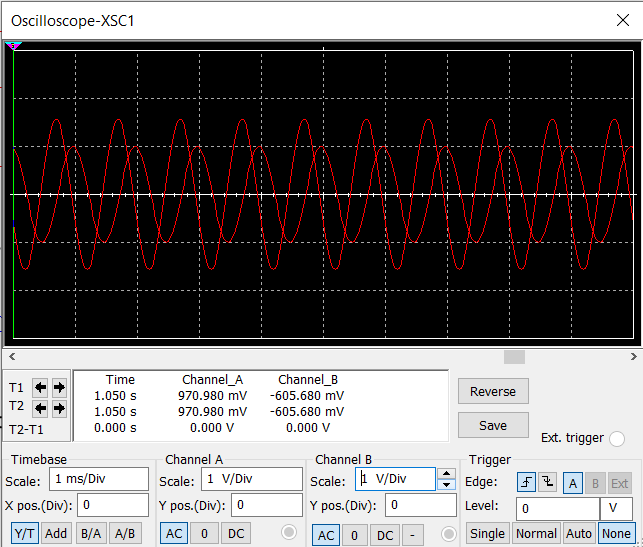
\includegraphics{images/intg sine.png}}

%*******************************************************************************%
%************************************START**************************************%
%*******************************************************************************%
\begin{document}

%************************************TITLE PAGE**************************************%
\begin{titlepage}
\begin{center}
\textbf{\LARGE Alexandria University}\\[0.5cm] 
\textbf{\large FACULTY OF ENGINEERING}\\[0.2cm]
\vspace{20pt}

\includegraphics{logo.png}\\[1cm]
\par
\vspace{20pt}
\textbf{\Large EEC332 Analog Integrated Circuits}\\
\vspace{15pt}
\myrule[1pt][7pt]
\textbf{\LARGE  Experiment 2}\\
\vspace{15pt}
\textbf{\large Study the characteristics of integrator and differentiator circuits}\\
\myrule[1pt][7pt]
\vspace{25pt}
\textbf{\large \hspace{50pt}Student Name \hspace{60pt} Student ID}\\
Ahmed Osama Mohamed Afifi \hspace{60pt} 20010038 \\
Ziad Mohamed Mohamed Abdalla \hspace{40pt} 20010643 \\

\vspace{45pt}
%\textbf {\large Lecturer in charge:}\\[0.2cm]
%\Large {Ir. Chan Cheong Loong}\\[0.1cm]
\end{center}

\par
\vfill
\begin{center}
\textbf{Submission Date : 18/04/2024}\\
\end{center}

\end{titlepage}

%************************************TABLE OF CONTENTS**************************************%

%  %Sumário
%  \newpage
%  \tableofcontents
%  \thispagestyle{empty}
%  %End Sumário

%********************************%
%***********SECTION 1************%
%********************************%
\newpage
\section{Introduction}
Integrators and differentiators can be used as a building block for filters. Filters form the essential block in analog signal processing to improve signal to noise ratio. An OP-Amp can be used to construct an integrator or a differentiator. This experiment is to understand the advantage of integrators as building blocks instead of differentiators. Differentiators are rejected because of their poor high-frequency noise response.
\newline

%********************************%
%***********SECTION 2************%
%********************************%
\section{Integrators}
\subsection{Schematic}
\begin{Figure}
 \centering
 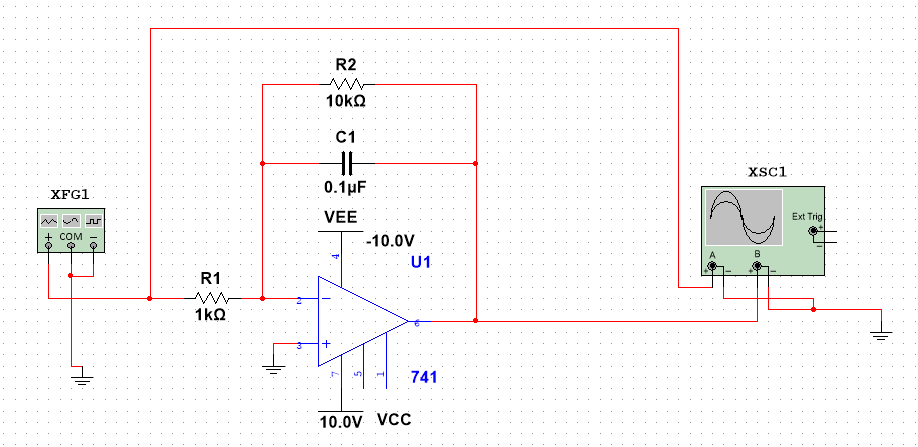
\includegraphics[width=1.2\linewidth, scale=2]{images/intg circuit.png}
 \captionof{figure}{Integrator}
\end{Figure}


\subsection{Results}

\subsubsection{Lab results}
\begin{figure}[H]
    \centering
    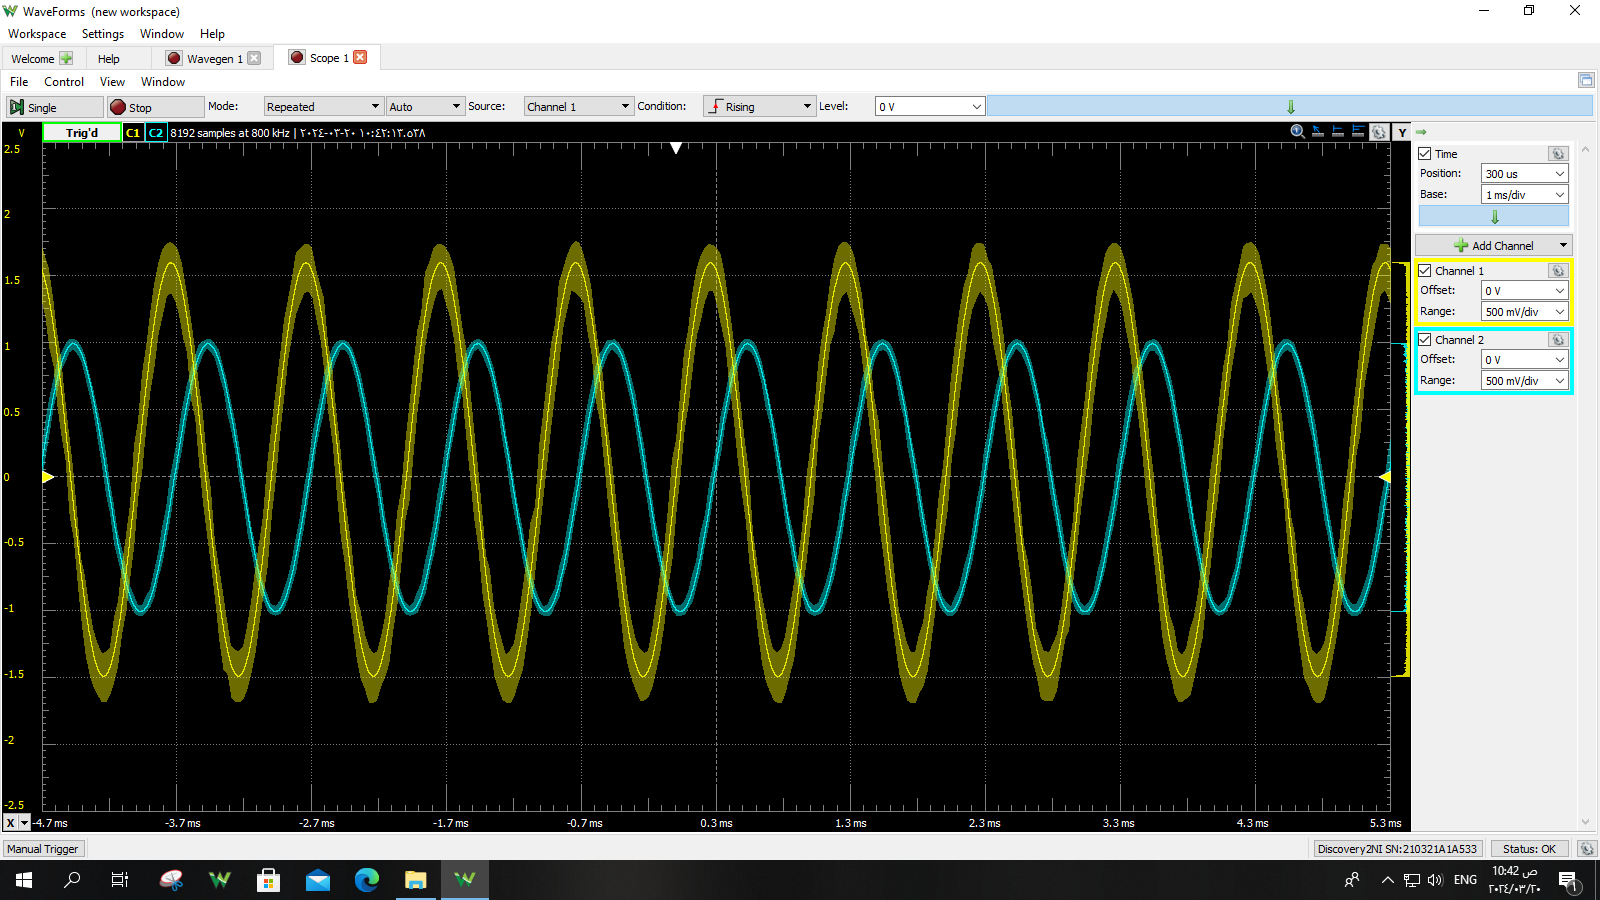
\includegraphics[width=\linewidth]{images/int sine lab.png}
    \caption{Lab result for integrator with sinusoidal wave input}
    \label{fig:Lab result for integrator with sinusoidal wave input}
\end{figure}
\begin{figure}[H]
    \centering
    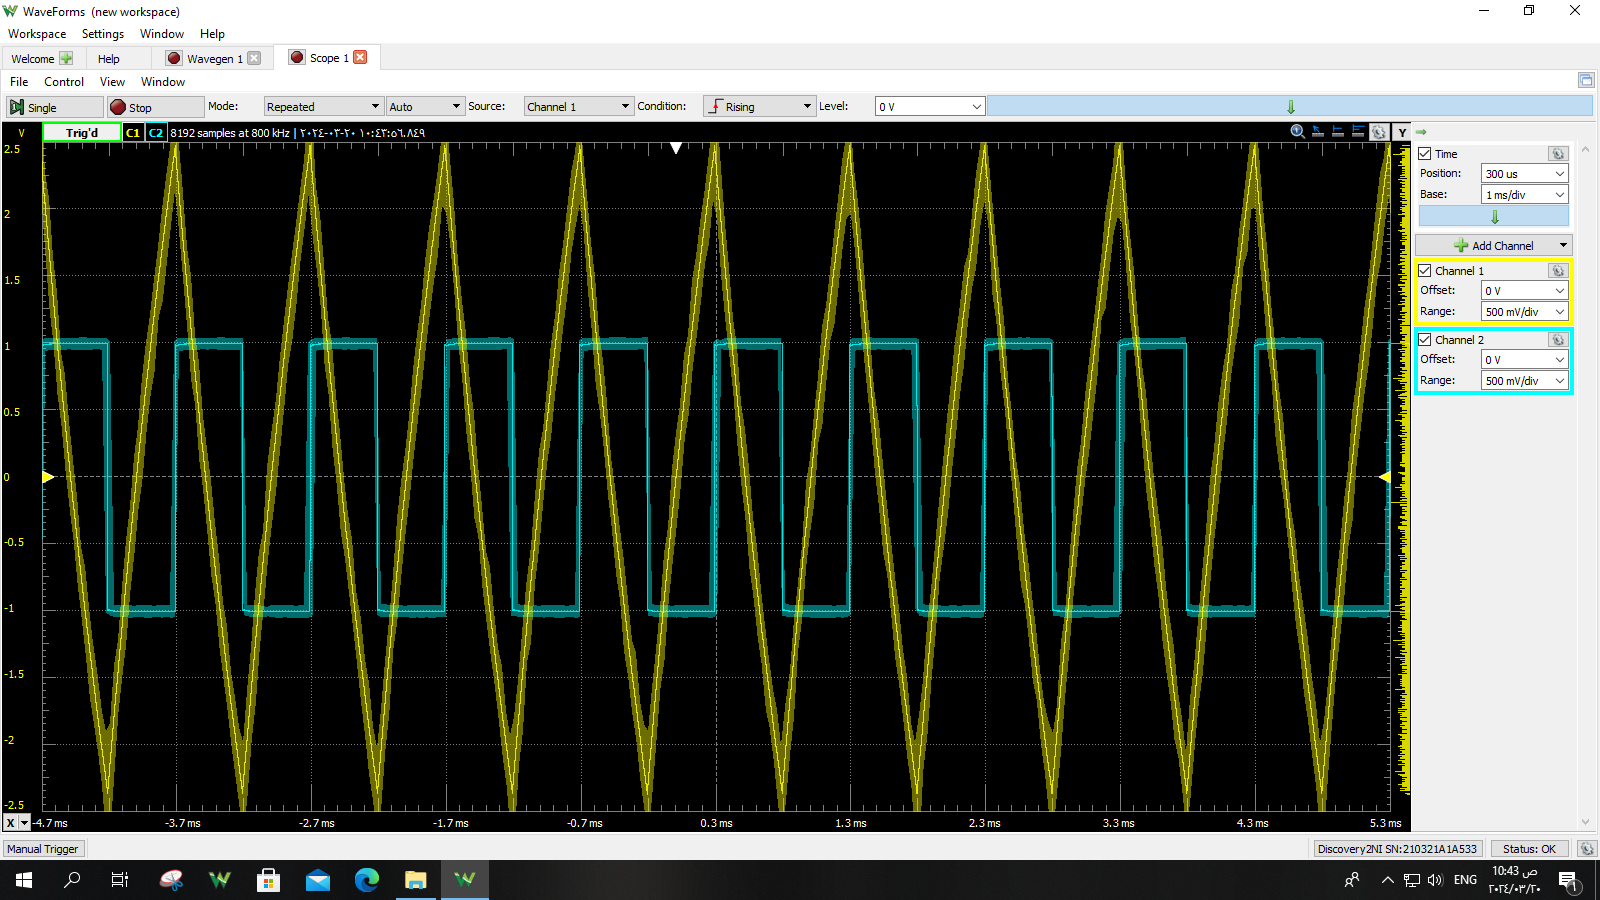
\includegraphics[width=\linewidth]{images/int square lab.png}
    \caption{Lab result for integrator with square wave input}
    \label{fig:Lab result for integrator with square wave input}
\end{figure}
\begin{figure}[H]
    \centering
    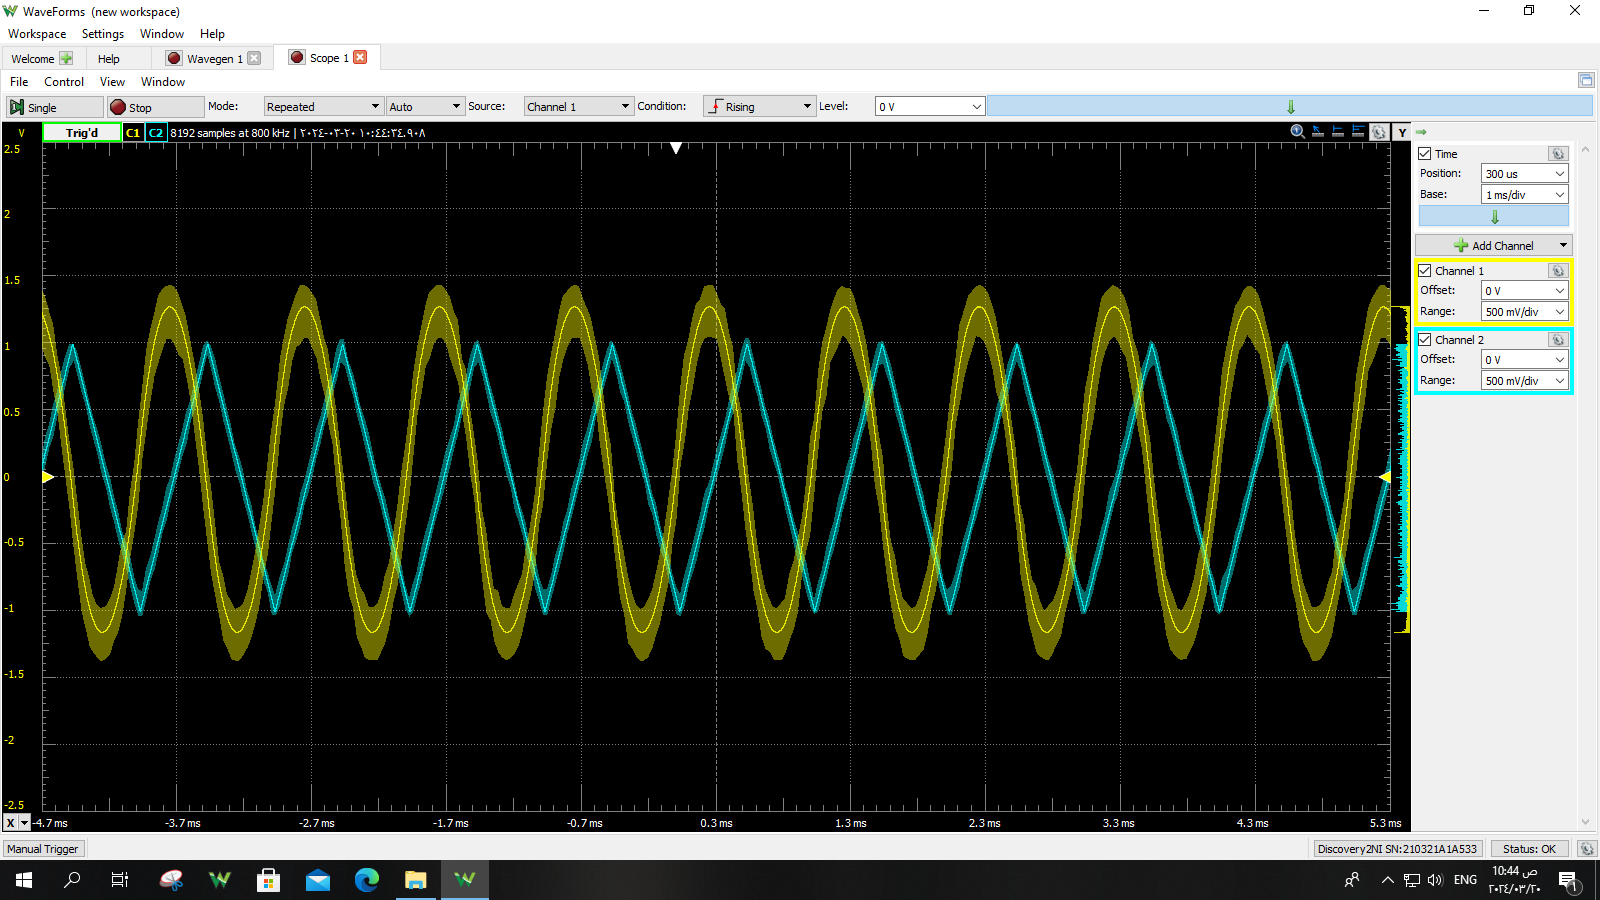
\includegraphics[width=\linewidth]{images/int tri lab.png}
    \caption{Lab result for integrator with triangular wave input}
    \label{fig:Lab result for integrator with triangular wave input}
\end{figure}


\subsubsection{Simulation results}
\begin{figure}[H]
    \centering
    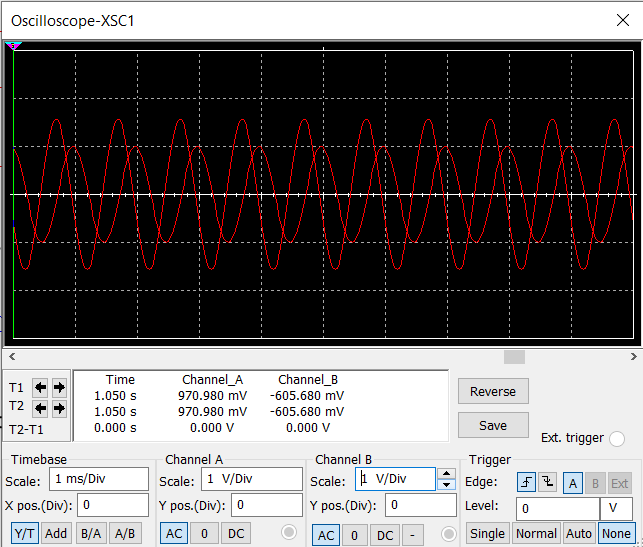
\includegraphics[width=\linewidth, height=0.8\simheight]{images/intg sine.png}
    \caption{Simulation result for integrator with sinusoidal wave input}
    \label{fig:Simulation result for integrator with sinusoidal wave input}
\end{figure}
\begin{figure}[H]
    \centering
    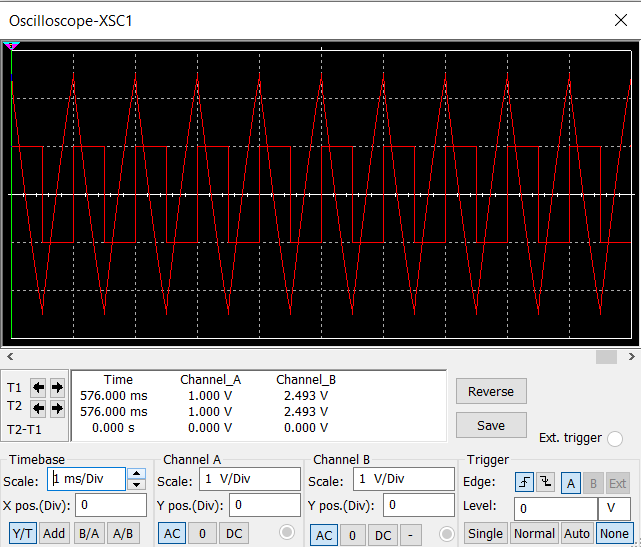
\includegraphics[width=\linewidth, height=0.8\simheight]{images/intg square.png}
    \caption{Simulation result for integrator with square wave input}
    \label{fig:Simulation result for integrator with square wave input}
\end{figure}
\begin{figure}[H]
    \centering
    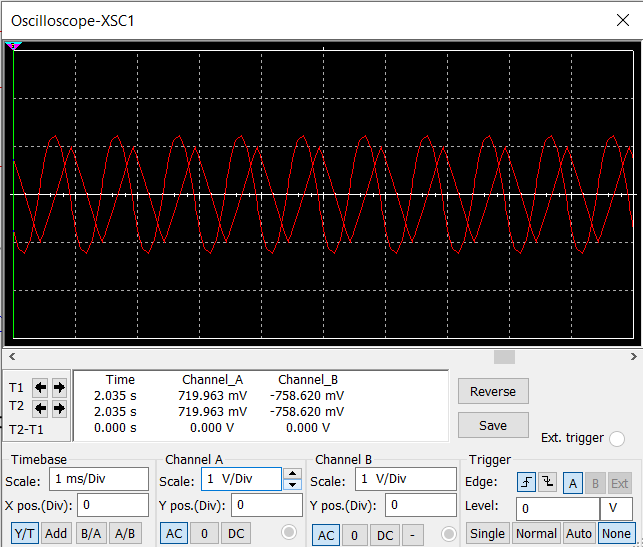
\includegraphics[width=\linewidth, height=0.8\simheight]{images/intg triangle.png}
    \caption{Simulation result for integrator with triangular wave input}
    \label{fig:Simulation result for integrator with triangular wave input}
\end{figure}

\begin{Figure}
 \centering
 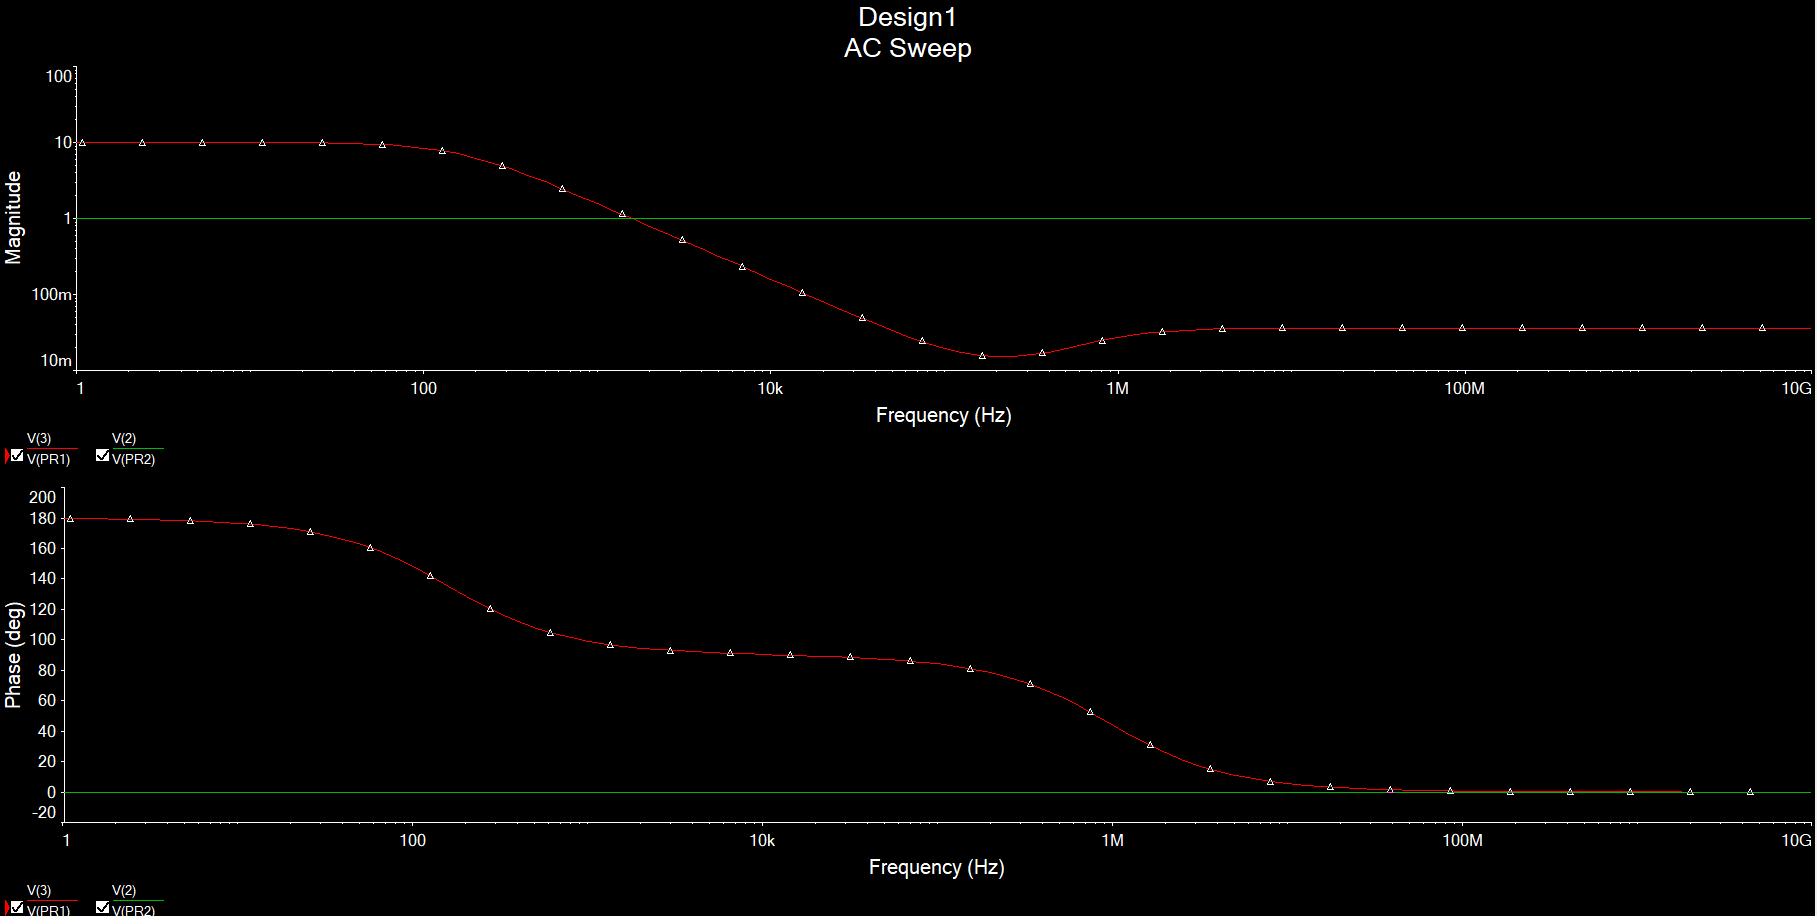
\includegraphics[width=\linewidth, scale=2]{images/intg freq res.png}
 \captionof{figure}{Frequency Response}
\end{Figure}

\subsection{Comments}
The integrator circuit produces an output signal that is the integral of the input signal. This can be noticed for the different input waveforms. It's important to note that the integrator's output amplitude and phase shift varied depending on the frequency and waveform of the input signal. Thus, it performs integration. One notable observation was that the integrator behaves as a low-pass filter and introduces a phase lag. This characteristic makes it suitable for applications such as signal conditioning and filtering.

\newpage
%********************************%
%***********SECTION 3************%
%********************************%
\section{Differentiators}
\subsection{Schematic}
\begin{Figure}
 \centering
 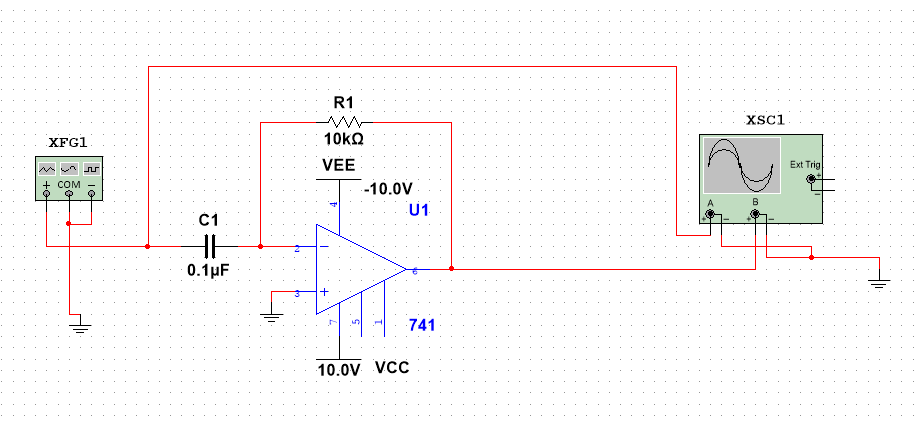
\includegraphics[width=1.2\linewidth, scale=2]{images/diff circuit.png}
 \captionof{figure}{Differentiator}
\end{Figure}


\subsection{Results}

\subsubsection{Lab results}
\begin{figure}[H]
    \centering
    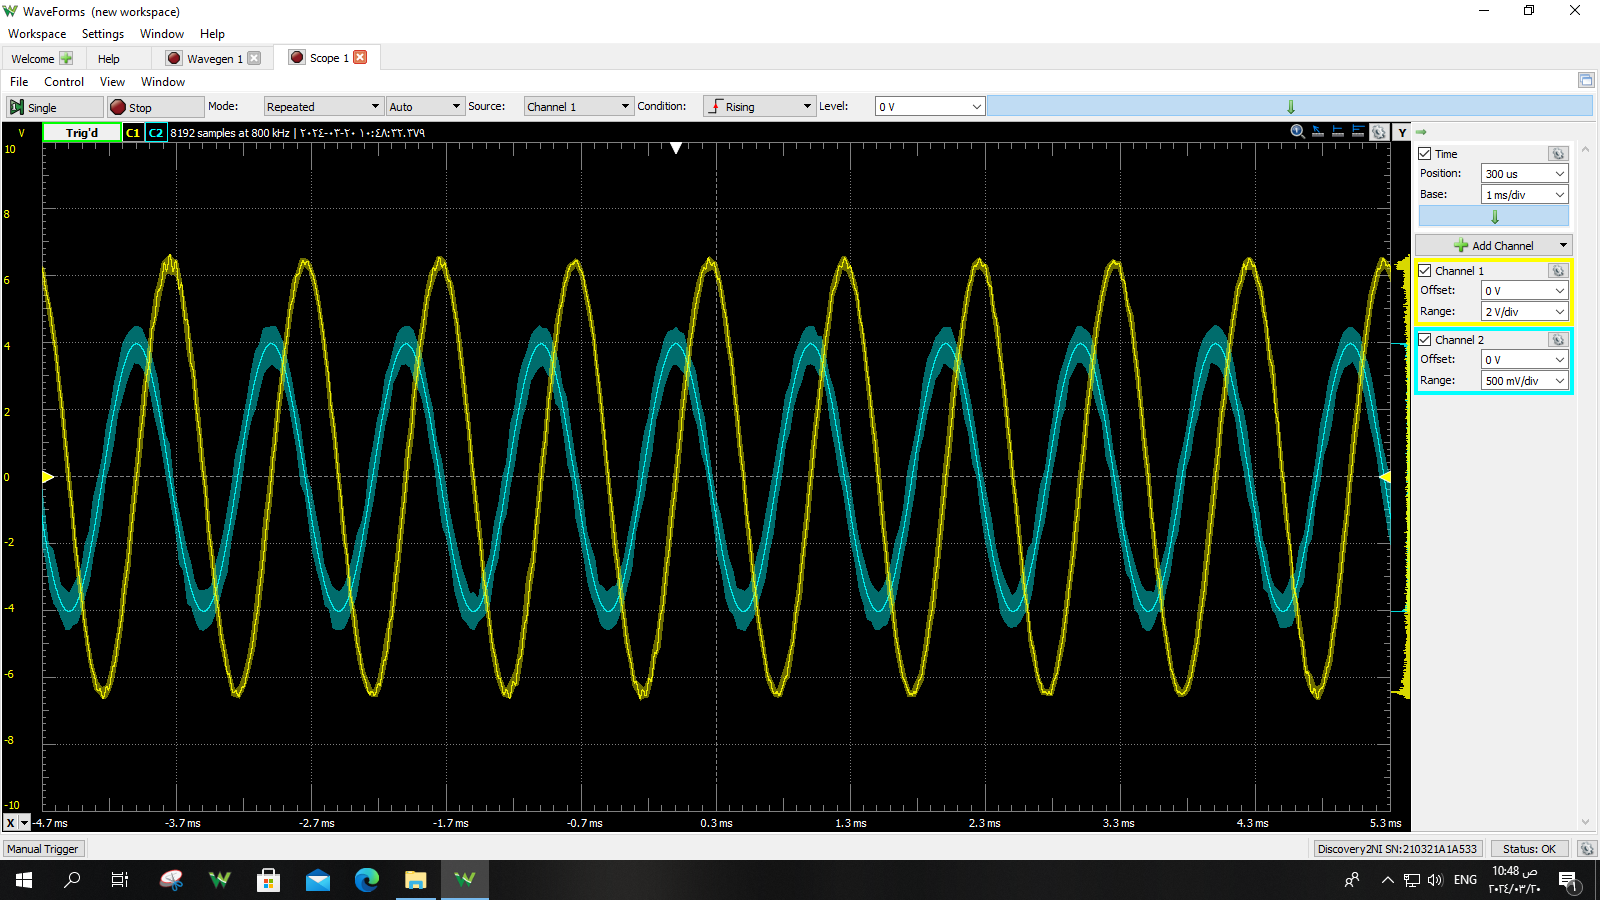
\includegraphics[width=\linewidth]{images/diff sine lab.png}
    \caption{Lab result for differentiator with sinusoidal wave input}
    \label{fig:Lab result for differentiator with sinusoidal wave input}
\end{figure}
\begin{figure}[H]
    \centering
    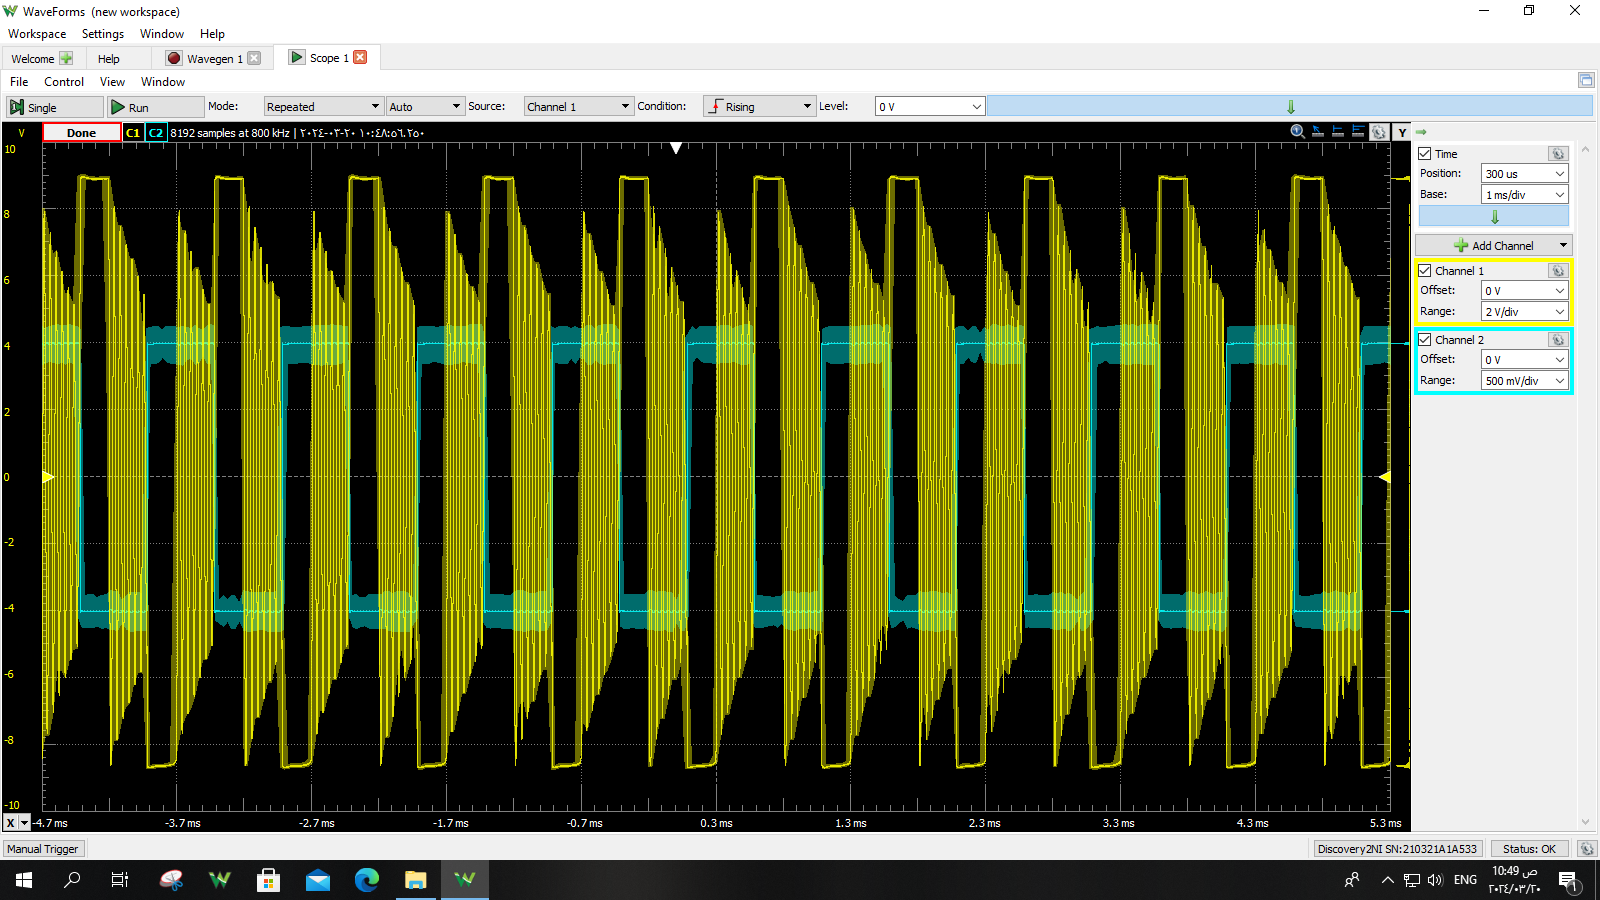
\includegraphics[width=\linewidth]{images/diff square lab.png}
    \caption{Lab result for differentiator with square wave input}
    \label{fig:Lab result for differentiator with square wave input}
\end{figure}
\begin{figure}[H]
    \centering
    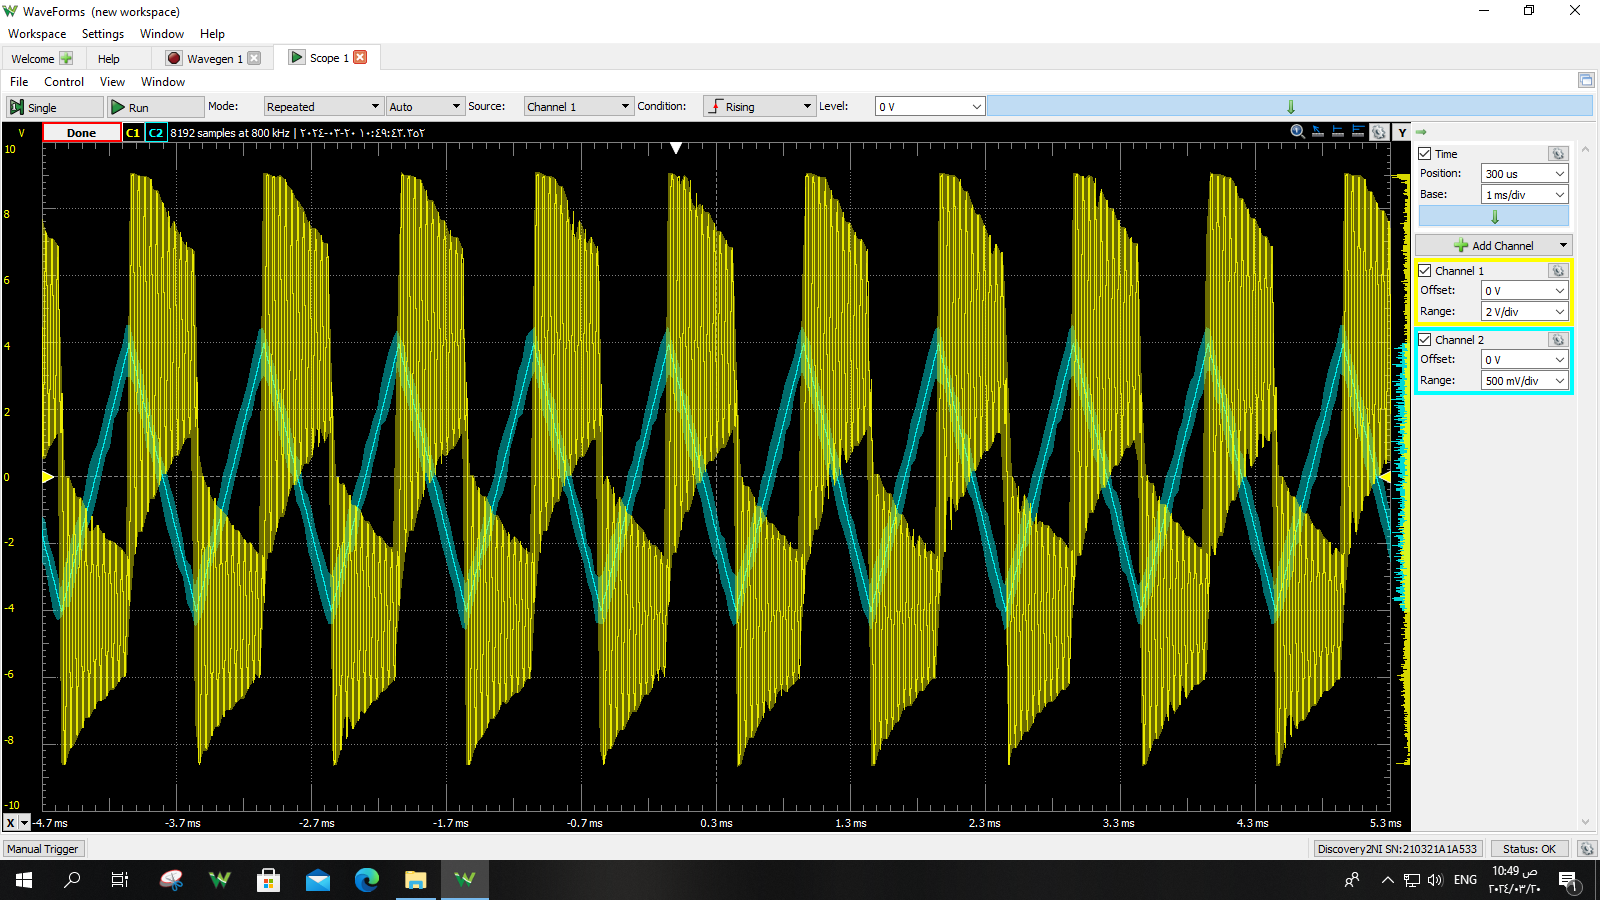
\includegraphics[width=\linewidth]{images/diff tri lab.png}
    \caption{Lab result for differentiator with triangular wave input}
    \label{fig:Lab result for differentiator with triangular wave input}
\end{figure}


\subsubsection{Simulation results}
\begin{figure}[H]
    \centering
    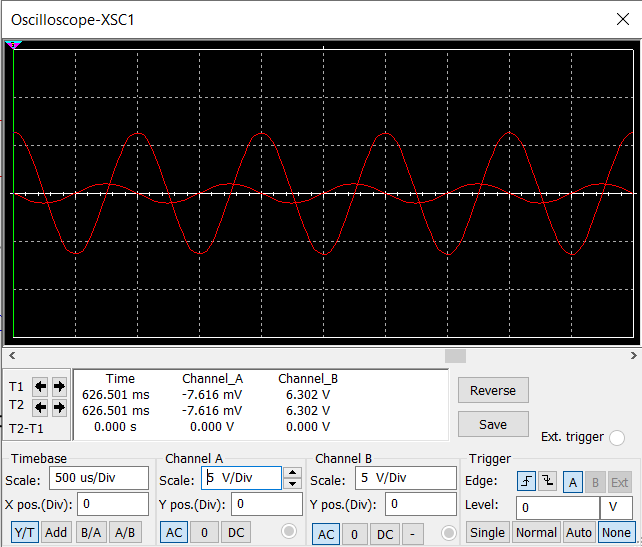
\includegraphics[width=\linewidth, height=0.8\simheight]{images/diff sine.png}
    \caption{Simulation result for differentiator with sinusoidal wave input}
    \label{fig:Simulation result for differentiator with sinusoidal wave input}
\end{figure}
\begin{figure}[H]
    \centering
    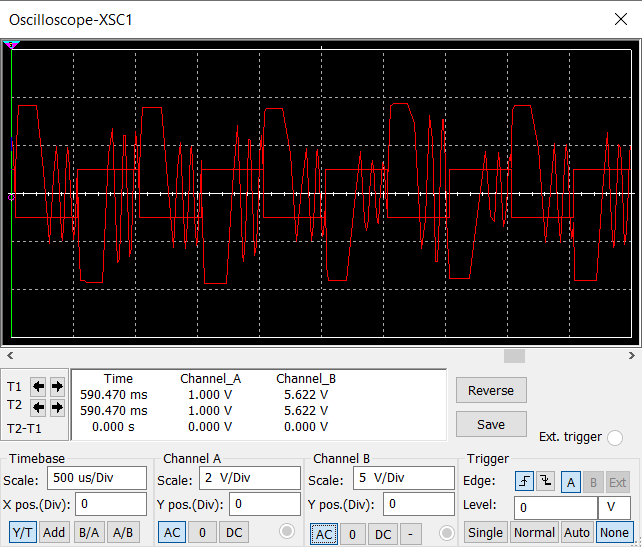
\includegraphics[width=\linewidth, height=0.8\simheight]{images/diff square.png}
    \caption{Simulation result for differentiator with square wave input}
    \label{fig:Simulation result for differentiator with square wave input}
\end{figure}
\begin{figure}[H]
    \centering
    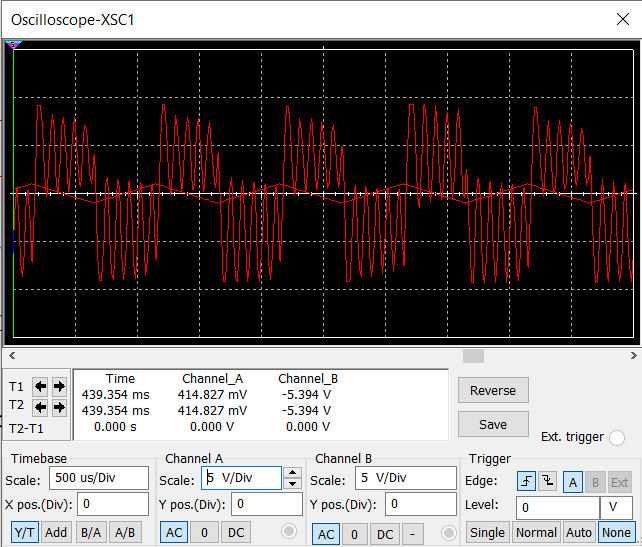
\includegraphics[width=\linewidth, height=0.8\simheight]{images/diff triangle.png}
    \caption{Simulation result for differentiator with triangular wave input}
    \label{fig:Simulation result for differentiator with triangular wave input}
\end{figure}

\begin{Figure}
 \centering
 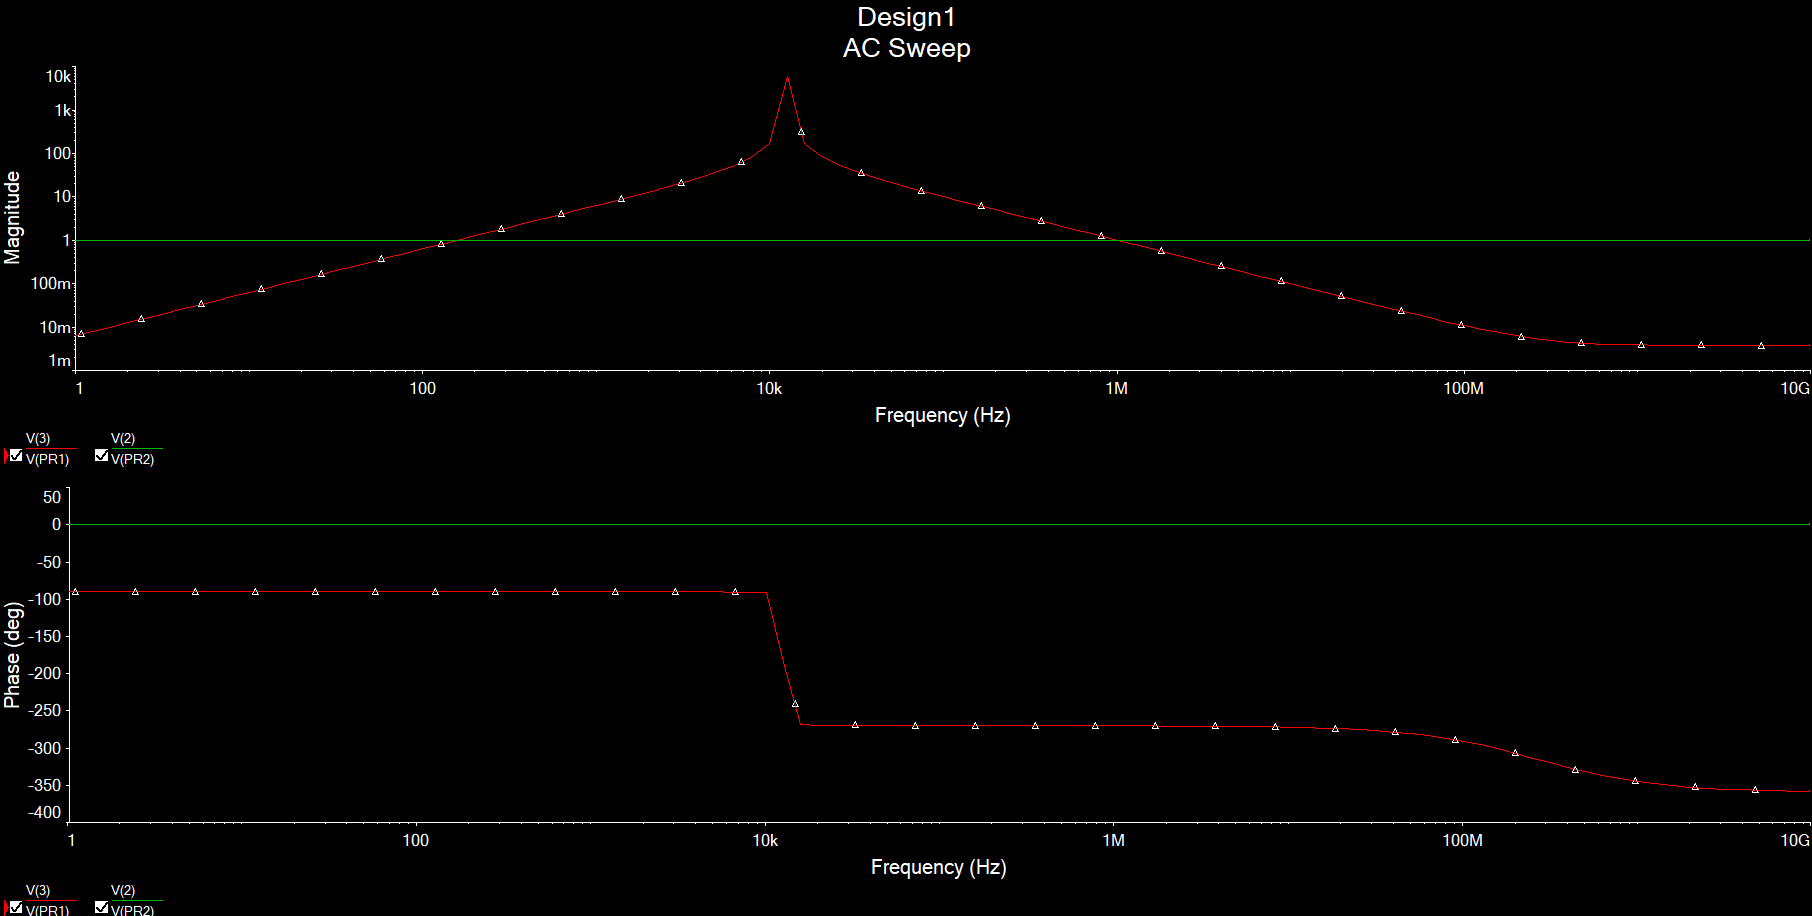
\includegraphics[width=\linewidth, scale=2]{images/diff freq res.png}
 \captionof{figure}{Frequency Response}
\end{Figure}

\subsection{Comments}
The differentiator circuit produces an output signal that is the derivative of the input signal. Similar to the integrator, the differentiator's response varied depending on the input waveform and frequency. One key observation is that the amplification of high-frequency components in the input signal by the differentiator. This behavior can be beneficial in applications where rapid changes in the input signal need to be detected. One notable observation was that the differentiator behaves as a high-pass filter.  Unlike the integrator, the differentiator circuit introduces a phase lead that becomes more pronounced at higher frequencies. Hence differentiator is sensitive to noise, filtering and signal conditioning, are necessary to minimize the impact of noise on the differentiator's performance.


\newpage

\patchcmd{\thebibliography}{\section*}{\section}{}{}

\end{document}